\section{Auswertung}
\label{sec:Auswertung}

\subsection{Fouriersynthese}

\subsubsection{Messwerte}
Die Rechteckspannung wird nach der $\frac{1}{k}$-Abhängigkeit mit den Amplituden
aus Tabelle \ref{tab:rechtampl} zusammengesetzt. Es werden nur die ungeraden
Oberwellen zugeschaltet.

\begin{table}[h]
  \centering
  \begin{tabular}{S S}
    \toprule
    {$k$} & {$U\:/\:\si{\milli\volt}$}\\
    \midrule
    1 & 637.2\\
    3 & 212.4\\
    5 & 127.4\\
    7 & 91.03\\
    9 & 70.8\\
    \bottomrule
  \end{tabular}
  \caption{Amplituden Rechteckspannung.}
  \label{tab:rechtampl}
\end{table}

Die Sägezahnspannung wird ebenfalls nach $\frac{1}{k}$-Abhängigkeit zusammengesetzt.
Allerdings werden diesmal auch die geraden Oberwellen zugeschaltet. Die
Amplituden der Spannungen sind in Tabelle \ref{tab:saegampl} aufgetragen.

\begin{table}[h]
  \centering
  \begin{tabular}{S S}
    \toprule
    {$k$} & {$U\:/\:\si{\milli\volt}$}\\
    \midrule
    1 & 637.2\\
    2 & 318.6\\
    3 & 212.4\\
    4 & 159.3\\
    5 & 127.4\\
    6 & 106.2\\
    7 & 91.03\\
    8 & 79.65\\
    9 & 70.8\\
    10 & 63.7\\
    \bottomrule
  \end{tabular}
  \caption{Amplituden Sägezahnspannung.}
  \label{tab:saegampl}
\end{table}

Die Dreiecksspannung wird nach einer $\frac{1}{k^2}$-Abhängigkeit zusammengesetzt.
Hier werden ebenso wie bei der Synthese der Rechtecksspannung nur die Oberwellen
ungeraden Indizes eingeschaltet. Die Amplituden der Spannungen sind in Tabelle \ref{tab:dreiampl}.

\begin{table}[h]
  \centering
  \begin{tabular}{S S}
    \toprule
    {$k$} & {$U\:/\:\si{\milli\volt}$}\\
    \midrule
    1 & 633.5\\
    3 & 70.4\\
    5 & 25.3\\
    7 & 12.9\\
    9 & 7.8\\
    \bottomrule
  \end{tabular}
  \caption{Amplituden Dreieckspannung.}
  \label{tab:dreiampl}
\end{table}

\subsubsection{Bilder der Spannungen}

Die Spannungen, die aus den oben angegeben Amplituden zusammengesetzt werden,
werden vom Oszilloskop gespeichert.

Das Oszilloskopbild zur Rechteckspannung wird in Abbildung
\ref{fig:oszrecht} gezeigt. Bei den Flanken sind gerade Linien
zu erkennen. Die oberen Linien zeigen noch klare Schwingungen.

\begin{figure}[h]
  \centering
  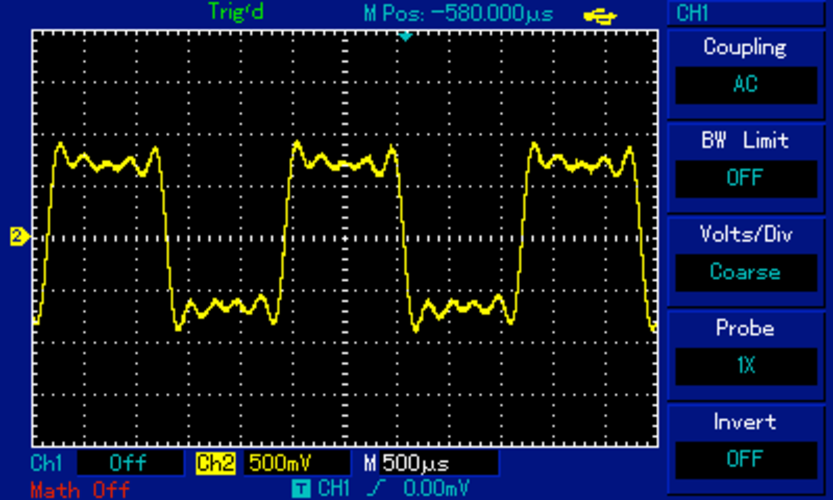
\includegraphics{oszrecht.pdf}
  \caption{Oszilloskopbild der synthetisierten Rechteckspannung.}
  \label{fig:oszrecht}
\end{figure}

Das Oszilloskopbild zur Sägezahnspannung wird in Abbildung \ref{fig:oszsaeg}
gezeigt. Die Flanken bestehen aus geraden Linien; die schrägen Abschnitte
sind stark von Schwingungen geprägt.

\begin{figure}[h]
  \centering
  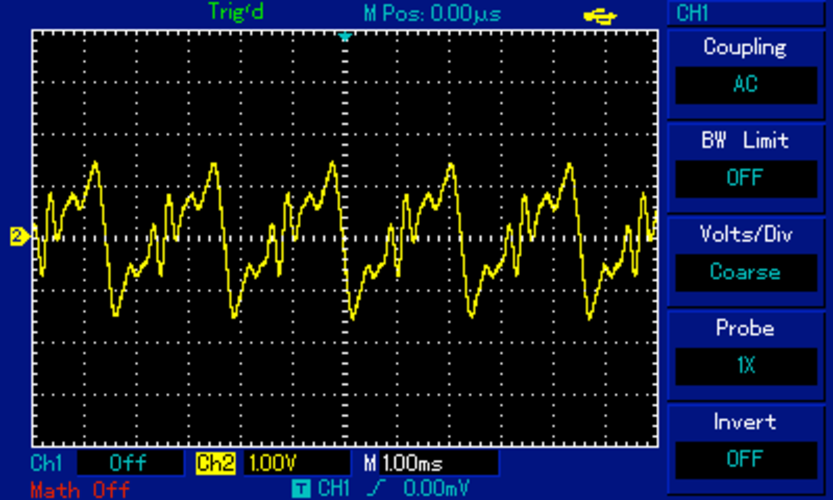
\includegraphics{oszsaeg.pdf}
  \caption{Oszilloskopbild der synthetisierten Saegezahnspannung.}
  \label{fig:oszsaeg}
\end{figure}

Das Oszilloskopbild zur Dreiecksspannung wird in Abbildung
\ref{fig:oszdrei} gezeigt. Die Dreieckform ist gut zu erkennen.

\begin{figure}[h]
  \centering
  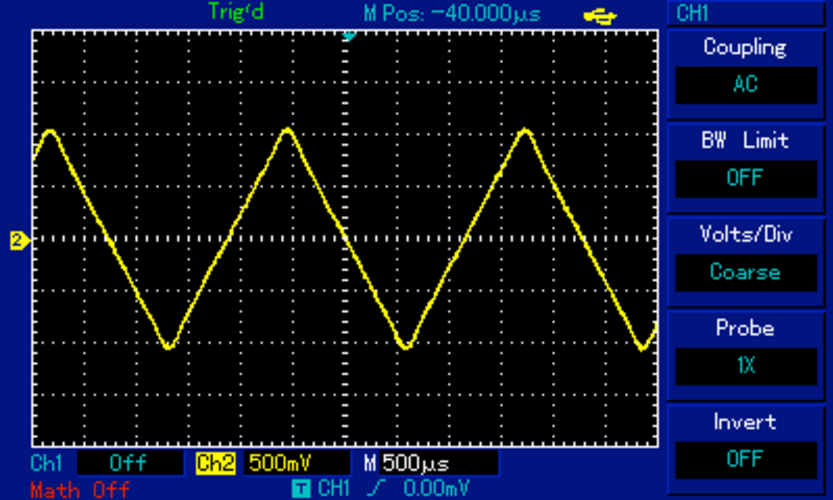
\includegraphics{oszdrei.pdf}
  \caption{Oszilloskopbild der synthetisierten Dreieckspannung.}
  \label{fig:oszdrei}
\end{figure}

\FloatBarrier

\subsection{Fourieranalyse}

%Rechteck
\begin{table}[h]
  \centering
  \begin{tabular}{S S S S}
    \toprule
    {$k$} & {$U_{\text{gem.}}\:/\:\si{\milli\volt}$}
     & {$U_{\text{theo.}}\:/\:\si{\milli\volt}$} & {$f\:/\:\si{\percent}$}\\
    \midrule
    1 & 2300 & 2300 & 0\\
    3 & 1350 & 767 & 76\\
    5 & 850 & 460 & 85\\
    7 & 560 & 329 & 70\\
    9 & 480 & 256 & 88\\
    11 & 350 & 209 & 67\\
    13 & 315 & 177 & 78\\
    15 & 220 & 153 & 43\\
    17 & 70 & 135 & 93\\
    \bottomrule
  \end{tabular}
  \caption{Amplituden Rechteckspannung nach Linienspektrum.}
  \label{tab:rechtanal}
\end{table}

In Tabelle \ref{tab:rechtanal} sind die gemessenen und theoretischen Amplituden
nach $\frac{1}{k}$-Abhängigkeit der Rechteckspannung eingetragen. Außerdem wird
die relative
Abweichung $f$ der gemessenen Amplitude vom theoretischen Wert angegeben.

Die Amplituden aus Tabelle \ref{tab:rechtanal} sind als Linienspektrum in
Abbildung \ref{fig:plotsprecht} eingezeichnet. Erwartet wird ein
$\frac{1}{k}$-Abfall der Linienspitzen. Dieser ist auch zu erkennen.

\begin{figure}[h]
  \centering
  \includegraphics{build/plotsprecht.pdf}
  \caption{Spektrum der Amplituden aus der Analyse der Rechteckspannung.}
  \label{fig:plotsprecht}
\end{figure}

%Sägezahn

\begin{table}[h]
  \centering
  \begin{tabular}{S S S S}
    \toprule
    {$k$} & {$U_{\text{gem.}}\:/\:\si{\milli\volt}$}
     & {$U_{\text{theo.}}\:/\:\si{\milli\volt}$} & {$f\:/\:\si{\percent}$}\\
    \midrule
    1 & 2100 & 2100 & 0\\
    2 & 950 & 1050 & 10\\
    3 & 700 & 700 & 0\\
    4 & 540 & 525 & 3\\
    5 & 420 & 420 & 0\\
    6 & 320 & 350 & 9\\
    7 & 280 & 300 & 7\\
    8 & 270 & 263 & 3\\
    9 & 240 & 233 & 3\\
    \bottomrule
  \end{tabular}
  \caption{Amplituden Sägezahnspannung nach Linienspektrum.}
  \label{tab:saeganal}
\end{table}

In Tabelle \ref{tab:saeganal} sind die gemessenen und theorethischen Amplituden
nach $\frac{1}{k}$-Abhängigkeit der Sägezahnspannung eingetragen. Außerdem wird
die relative
Abweichung $f$ der gemessenen Amplitude vom theoretischen Wert angegeben.

Die Amplituden aus Tabelle \ref{tab:saeganal} sind als Linienspektrum in
Abbildung \ref{fig:plotspsaeg} eingezeichnet. Erwartet wird ein
$\frac{1}{k}$-Abfall der Linienspitzen. Dieser ist auch zu erkennen. Die
letzten Werte fallen allerdings etwas zu leicht ab.

\begin{figure}[h]
  \centering
  \includegraphics{build/plotspsaeg.pdf}
  \caption{Spektrum der Amplituden zur Analyse der Sägezahnspannung.}
  \label{fig:plotspsaeg}
\end{figure}

%Dreieck

\begin{table}[h]
  \centering
  \begin{tabular}{S S S S}
    \toprule
    {$k$} & {$U_{\text{gem.}}\:/\:\si{\milli\volt}$}
     & {$U_{\text{theo.}}\:/\:\si{\milli\volt}$} & {$f\:/\:\si{\percent}$}\\
    \midrule
    1 & 2700 & 2700 & 0\\
    3 & 300 & 300 & 0\\
    5 & 110 & 108 & 2\\
    7 & 48 & 55 & 13\\
    9 & 26 & 33 & 22\\
    11 & 18 & 22 & 19\\
    13 & 17 & 16 & 6\\
    15 & 9 & 12 & 25\\
    17 & 5 & 9 & 46\\
    \bottomrule
  \end{tabular}
  \caption{Amplituden Dreieckspannung nach Linienspektrum.}
  \label{tab:dreianal}
\end{table}

In Tabelle \ref{tab:dreianal} sind die gemessenen und theorethischen Amplituden
nach $\frac{1}{k^2}$-Abhängigkeit der Dreieckspannung eingetragen. Außerdem wird
die relative
Abweichung $f$ der gemessenen Amplitude vom theoretischen Wert angegeben.

Die Amplituden aus Tabelle \ref{tab:dreianal} sind als Linienspektrum in
Abbildung \ref{fig:plotspdrei} eingezeichnet. Erwartet wird ein
$\frac{1}{k^2}$-Abfall der Linienspitzen. Dieser ist auch zu erkennen.

\begin{figure}[h]
  \centering
  \includegraphics{build/plotspdrei.pdf}
  \caption{Spektrum der Amplituden zur Analyse der Dreiecksspannung.}
  \label{fig:plotspdrei}
\end{figure}
